\documentclass[12pt,letterpaper]{article}
\usepackage[utf8]{inputenc}
\usepackage[spanish,es-tabla]{babel}
\decimalpoint
\let\cleardoublepage\clearpage
\usepackage[bitstream-charter]{mathdesign} 
\usepackage[T1]{fontenc}
\newcommand{\selectSans}{\usefont{T1}{qhv}{m}{n}\selectfont} % sans-serif TeX Gyre Heros font
\usepackage{amsmath}
\usepackage{amsfonts}
\usepackage{amssymb}
% \usepackage[T1]{fontspec}
\usepackage{color}
\usepackage{graphicx}
\usepackage{makeidx}
\makeindex
\usepackage{anysize}
\usepackage{anyfontsize}
\usepackage{pdfpages}
\usepackage[x11names,table]{xcolor}
\usepackage{tikz}
\usepackage{tcolorbox}
\tcbuselibrary{skins,breakable,listings,theorems}
\usepackage[hidelinks]{hyperref}
\usepackage[labelfont=bf]{caption}
\captionsetup[table]{labelsep=space}
\captionsetup[figure]{labelsep=space}
\usepackage{listings}
\usepackage{array,ragged2e}
\usepackage{multirow}
\usepackage[left=2cm,top=2cm,right=2cm,bottom=2cm]{geometry}
\setlength{\parindent}{0cm}
% \usepackage[printwatermark]{xwatermark}
% \newwatermark[allpages,color=gray!10,angle=45,scale=3,xpos=0,ypos=0]{Borrador}

\tcbset{colback=green!5!white, colframe=gray!10!black, coltitle=green!20!black, 
fonttitle=\bfseries, colbacktitle=white, coltext=gray!30!black}
\addto\captionsspanish{
  \renewcommand{\figurename}{{\bf Figura}}% 
}
\addto\captionsspanish{
  \renewcommand{\chaptername}{{\bf}}% 
}

\usepackage{epigraph}
\usepackage{fontawesome}
\usepackage[Bjornstrup]{fncychap}

% \renewcommand{\familydefault}{\sfdefault}

% Colores
\definecolor{verdep}{RGB}{166,206,58}
\definecolor{ccap}{RGB}{10,10,50}
\definecolor{csec}{RGB}{50,50,100}
\definecolor{csubsec}{RGB}{80,80,120}
\definecolor{header_table_color}{RGB}{200,255,180}
\definecolor{info_color}{RGB}{100,100,200}
\definecolor{csol}{rgb}{0.2,0.8,0.1}
\definecolor{backcode}{rgb}{0.98,0.98,0.99}
\definecolor{crule}{rgb}{0.9,0.9,0.9}
\definecolor{dkgreen}{rgb}{0,0.6,0}
\definecolor{gray}{rgb}{0.5,0.5,0.5}
\definecolor{mauve}{rgb}{0.58,0,0.82}


\newtcolorbox{ejemplo}[2][]
{
  breakable,
  colframe = gray!50,
  colback  = gray!0,
  coltitle = gray!20!black,
  title    =  \faEdit \hspace{5 mm} #2,
}

\newtcolorbox{informacion}[2][]
{
  breakable,
  colframe = blue!5!white,
  colback  = blue!5!white,
  coltitle = blue!80!black,
  title    = \faInfo \hspace{5 mm} #2,
}

\newtcolorbox{recomendacion}[2][]
{
  breakable,
  colframe = green!25,
  colback  = green!10,
  coltitle = green!20!black,
  title    = #2,
}

 \newcommand{\ccol}{>{\centering\tt\arraybackslash}}

% Nuevos comandos

\usepackage{titlesec}%--
% \newcommand{\hsp}{\hspace{5pt}}
% \titleformat{\chapter}[hang]{\huge\bfseries\color{ccap}}
% {\color{verdep}{\vrule height 2.5cm width 1mm}\hsp{\fontsize{100}{5}\selectfont\thechapter}\hsp%
% {\vrule height 2.5cm width 1mm}\hsp{\fontsize{30}{5}\selectfont}}{5pt}{\huge\bfseries}

\titleformat{\section}[hang]{\normalfont\color{csec}}%
{\filright\large\enspace\thesection\enspace}%
{8pt}{\Large\bfseries\filright}%

\titleformat{\subsection}[hang]{\normalfont\color{csec}}%
{\filright\large\enspace\thesubsection\enspace}%
{8pt}{\large\bfseries\filright}%

% Code
\lstnewenvironment{matlab}{\lstset{frame=single,
  frameround=tttt,
  backgroundcolor=\color{backcode},
  rulecolor=\color{crule},
  language=matlab,
  aboveskip=5mm,
  belowskip=5mm,
  showstringspaces=false,
  columns=flexible,
  basicstyle={\small\ttfamily},
  numbers=none,
  numberstyle=\tiny\color{gray},
  keywordstyle=\color{blue},
  commentstyle=\color{dkgreen},
  stringstyle=\color{mauve},
  breaklines=true,
  breakatwhitespace=true,
  tabsize=4,
  extendedchars=true,
  inputencoding=utf8,
  literate=%
  {°}{{\,\,$^\circ$\,\,}}1
  {á}{{\'a}}1
  {é}{{\'e}}1
  {í}{{\'i}}1
  {ó}{{\'o}}1
  {ú}{{\'u}}1
  {Á}{{\'A}}1
  {É}{{\'E}}1
  {Í}{{\'I}}1
  {Ó}{{\'O}}1
  {Ú}{{\'U}}1
}}{}


\author{Pedro Jorge De Los Santos}
\title{
{\bf\Large Apuntes de Mecánica de Materiales} \\
{\large I. Esfuerzo y deformación}
}

% =================================================================
% =================================================================
%                              CONTENIDO
% =================================================================
% =================================================================

\begin{document}
\maketitle
\tableofcontents

\section{Introducción a la mecánica de materiales}

La mecánica de materiales \footnote{También conocida como Resistencia de Materiales} es una rama de la 
mecánica aplicada que estudia el comportamiento de cuerpos sólidos sometidos a diversas cargas, incluyendo 
en esta definición a todo tipo de elementos estructurales: barras, columnas, vigas, armaduras, ejes; sometidos a 
diversas configuraciones de carga: axiales, a torsión, compresión y/o una combinación de las anteriores. \\

El objetivo principal de la mecánica de materiales es determinar los esfuerzos, las deformaciones 
unitarias y los desplazamientos en estructuras y sus componentes debidas a las cargas que actúan sobre 
ellas. Si podemos determinar estas cantidades para todos los valores de las cargas incluyendo las 
que causan la falla, tendremos una representación completa del comportamiento mecánico de esas estructuras. \\

Entender el comportamiento mecánico es esencial para el diseño seguro de todos los tipos de estructuras, ya sean 
elementos de una maquinaria, edificios, puentes. Esta es la razón por la cual la mecánica de materiales es una 
disciplina básica en muchos campos de la ingeniería. Los análisis teóricos y los resultados experimentales 
desempeñan papeles igualmente importantes en la mecánica de materiales. Empleamos teorías para deducir fórmulas 
y ecuaciones para predecir el comportamiento mecánico, pero no se pueden usar estas expresiones en un diseño 
práctico, a menos que se conozcan las propiedades físicas de los materiales. Esas propiedades se conocen 
sólo después de que se han efectuados experimentos cuidadosos en el laboratorio.


\section{Esfuerzo normal y deformación unitaria}

Los conceptos fundamentales de esfuerzo y deformación pueden ser ilustrados considerando una barra 
prismática cargada axialmente con una fuerza P en sus extremos, como se muestra en la figura 
\ref{fig:barra_prismatica}. Una barra prismática es un elemento estructural recto que tiene una 
misma sección transversal a lo largo de su longitud. La fuerza axial produce un estrechamiento uniforme 
en la barra, en este caso se dice que la barra está a tensión.

\begin{center}
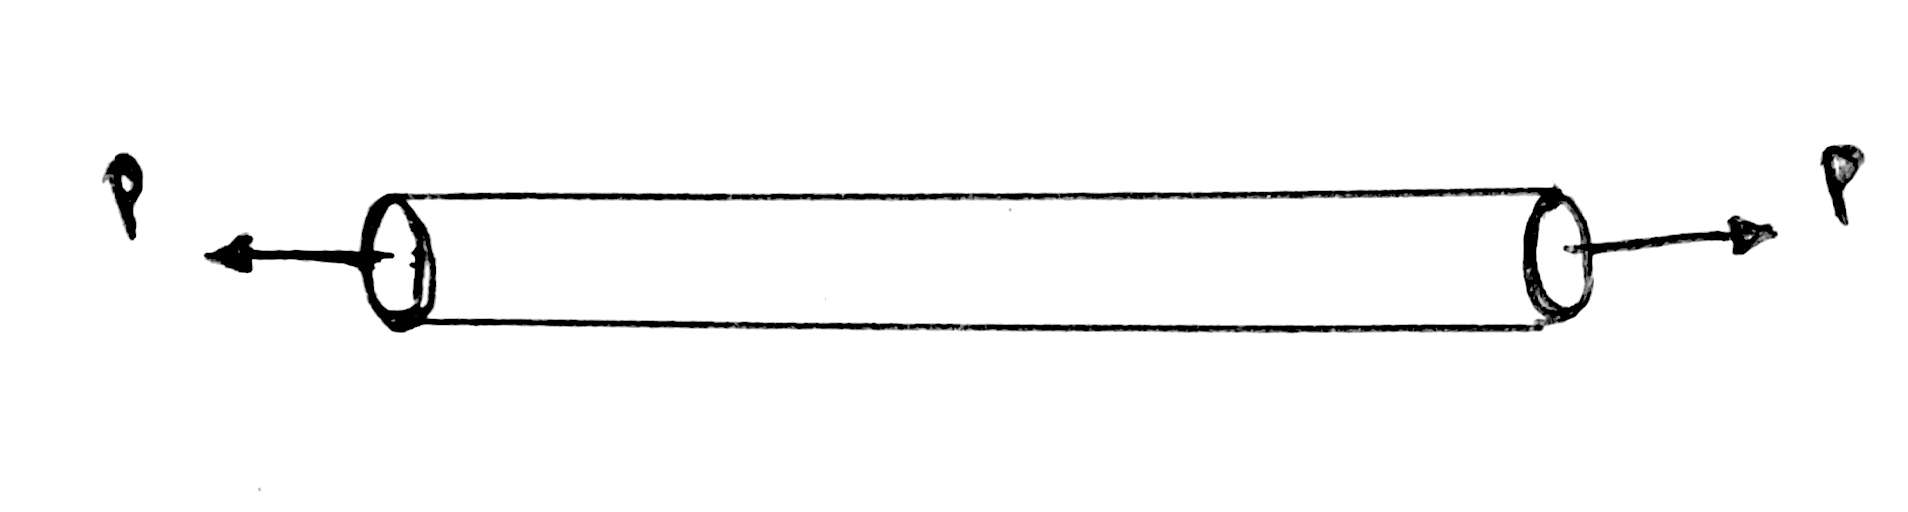
\includegraphics[width=0.35\textwidth]{img/barra_prismatica.jpg}
\captionof{figure}{Barra prismática}
\label{fig:barra_prismatica}
\end{center}

Para determinar los esfuerzos y deformaciones en esta barra , consideremos 
los diagramas mostrados en la figura \ref{fig:barra_tension}, el primero referente a una barra de longitud L antes de 
que las cargas sean aplicadas, y el otro a una barra deformada después que las cargas son aplicadas. Los esfuerzos 
internos producidos por las fuerzas axiales ($P$) pueden mostrarse si hacemos un corte imaginario en la sección 
$mn$. Ahora aislamos la parte de la barra a la izquierda de la sección transversal $mn$ como un cuerpo libre, 
(como se muestra en el tercer diagrama) en el extremo derecho de este cuerpo libre mostramos la acción de la 
parte eliminada de la barra. Esta acción consiste en esfuerzos distribuidos en forma continua que actúan sobre 
toda la sección transversal y la fuerza axial $P$ que actúa en la sección transversal es la resultante de estos 
esfuerzos.

\begin{center}
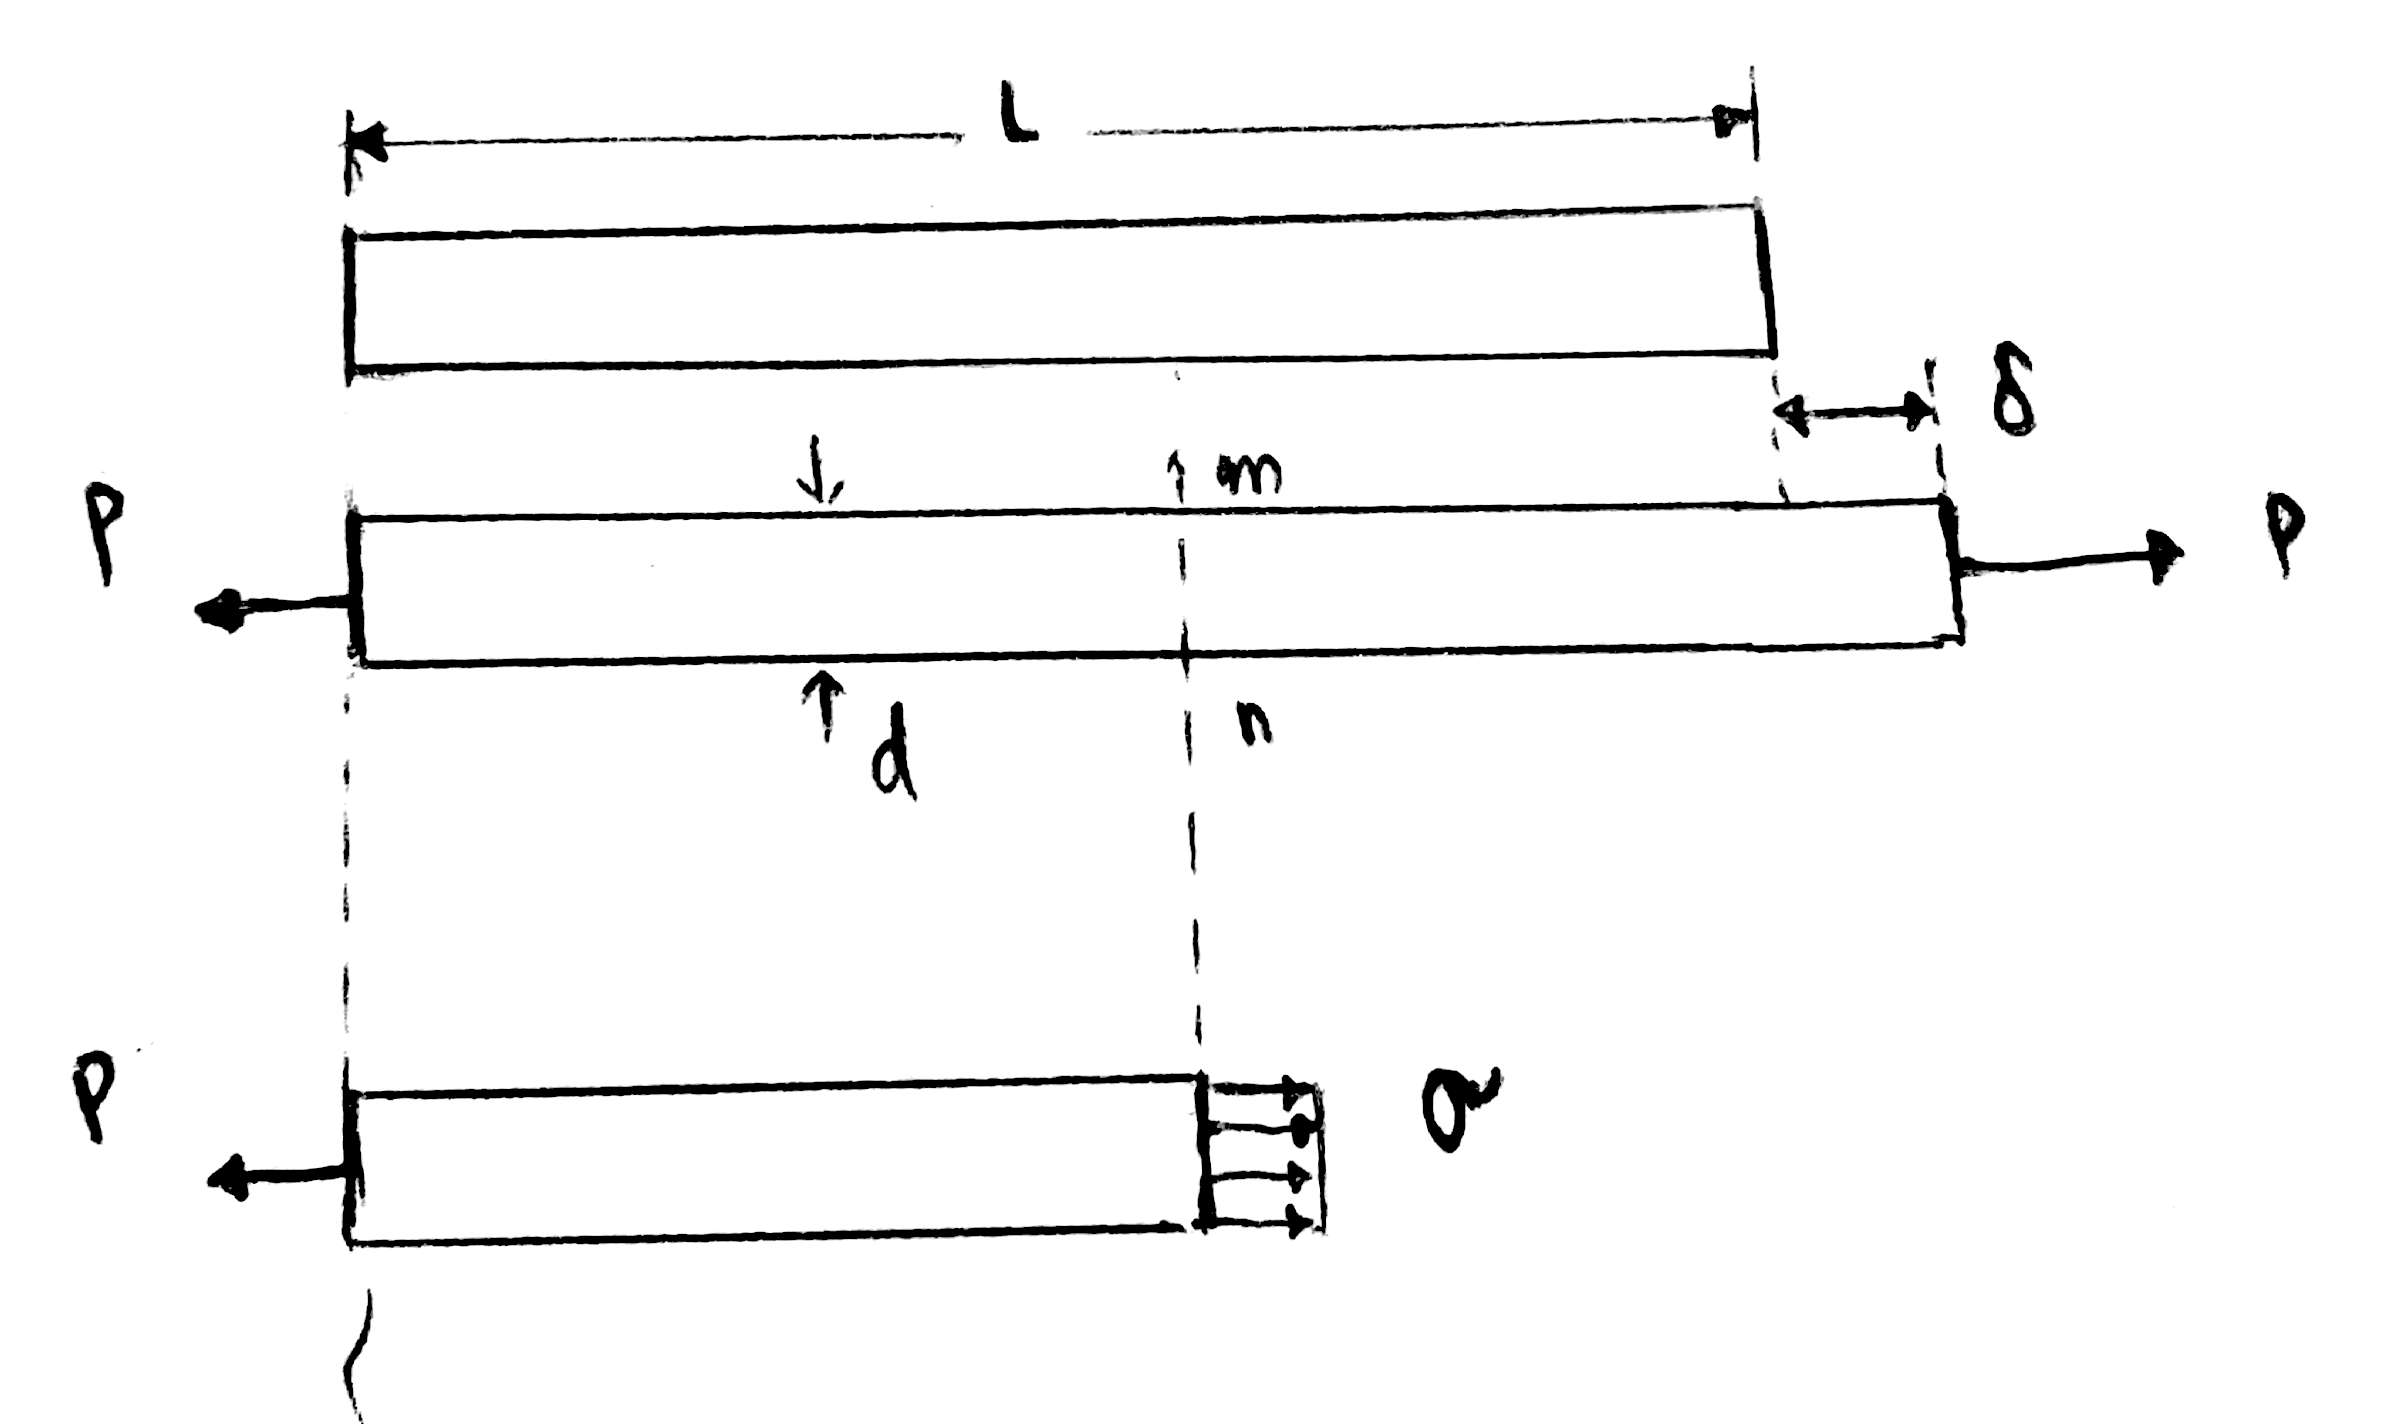
\includegraphics[width=0.55\textwidth]{img/barra_tension.jpg}
\captionof{figure}{Barra prismática sometida a tensión}
\label{fig:barra_tension}
\end{center}

El esfuerzo tiene unidades de fuerza por unidad de área y se denota por la letra griega sigma ($\sigma$), en general, 
los esfuerzos $\sigma$ que actúan sobre una superficie plana pueden ser uniformes en toda el área o bien variar 
en intensidad de un punto a otro. Supongamos que los esfuerzos que actúan sobre la sección transversal $mn$ están 
distribuidos uniformemente sobre el área, entonces la resultante de estos esfuerzos deben ser igual a la magnitud del 
esfuerzo por el área de la sección transversal $A$ de la barra, es decir, $P = \sigma A$. Por tanto, obtenemos la 
expresión siguiente para la magnitud de los esfuerzos:

\begin{equation}
\sigma = \frac{P}{A}
\end{equation}

Esta ecuación expresa la intensidad de un esfuerzo uniforme en una barra prismática con sección transversal arbitraria 
cargada axialmente.\\

Cuando la barra es estirada por las fuerzas $P$, los esfuerzos son esfuerzos de tensión; si se invierte la dirección 
de las fuerzas, la barra se comprime y tenemos esfuerzos de compresión. Puesto que los esfuerzos actúan en una 
dirección perpendicular a la superficie cortada, se denominan esfuerzos normales. Y, por tanto, los esfuerzos normales 
pueden ser de tensión o compresión.\\

\begin{informacion}{Convención de signos de los esfuerzos}
Cuando se requiere una convención de signos para los esfuerzos normales, se acostumbra a definir los esfuerzos de tensión 
como positivos y a los esfuerzos de compresión como negativos.
\end{informacion} \hfill \\

Una barra cargada axialmente presenta un cambio de longitud: comprimiéndose o alargándose dependiendo del tipo 
de esfuerzo inducido. El cambio en la longitud se denota con la letra griega $\delta$.\\

En general, el alargamiento de un segmento es igual a su longitud dividida entre la longitud total $L$ y multiplicada 
por el alargamiento $\delta$. Por tanto, una longitud unitaria de la barra tendrá un alargamiento igual a $1/L$ por 
$\delta$. Esta cantidad se denomina \textbf{deformación unitaria} y se denota con la letra griega $\epsilon$. Podemos 
observar que la deformación unitaria está dada por la ecuación:

\begin{equation}
\epsilon = \frac{\delta}{L}
\end{equation}

Si la barra está a tensión, la deformación unitaria se denomina deformación unitaria por tensión, que representa 
un alargamiento o estiramiento del material. Si la barra está en compresión, la deformación unitaria es una deformación 
unitaria por compresión y la barra se acorta. En general, la deformación unitaria por tensión se considera positiva 
y la deformación unitaria por compresión como negativa. Como la deformación unitaria es la razón de dos longitudes, es 
una cantidad adimensional, es decir, no tiene unidades. Los valores numéricos de la deformación 
unitaria suelen ser muy pequeños, debido a que las barras hechas de material estructural sólo experimentan cambios 
muy pequeños de longitud cuando se someten a cargas. \\

\begin{ejemplo}{Ejemplo 1}

Una barra prismática con sección transversal rectangular como se muestra en la figura, está sujeta a 
una carga axial a tensión $P$. La elongación medida en la barra es de $\delta = 1.2 \,\, \text{mm}$. 
Calcular el esfuerzo normal y la deformación unitaria en la barra, sabiendo que $L = 3\,\text{m} $, 
$P = 50 \, \text{kN}$, $a=20 \, \text{mm}$ y $b=40 \, \text{mm}$.

\begin{center}
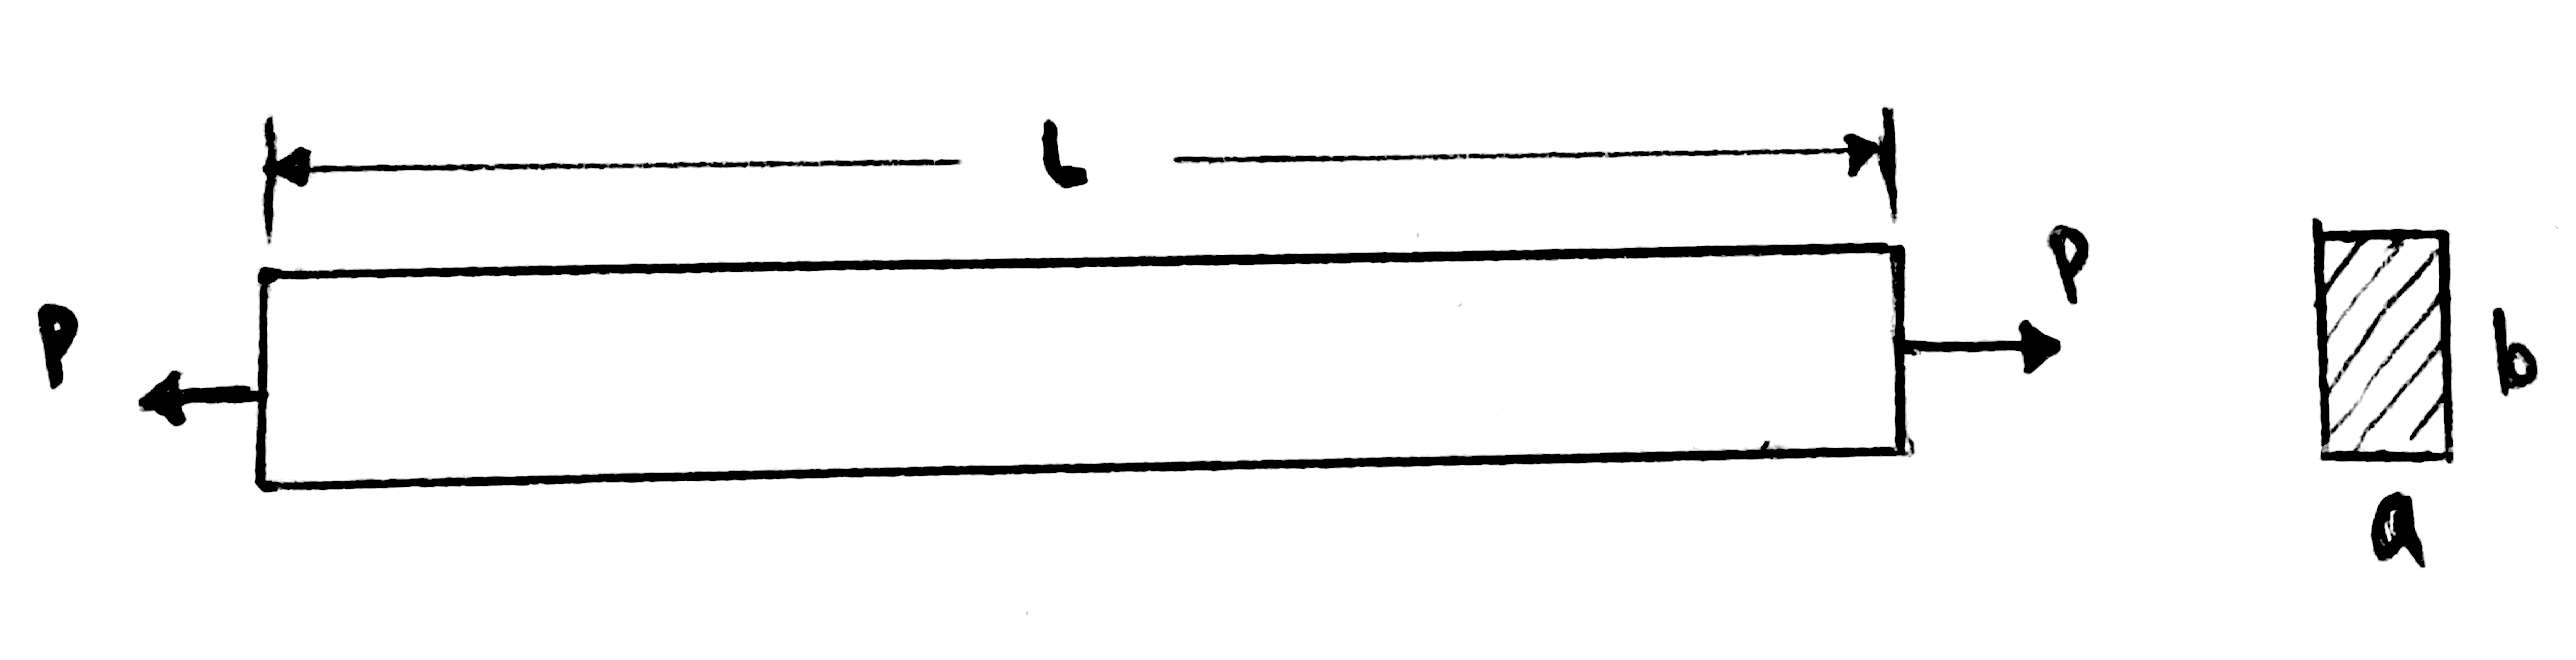
\includegraphics[width=0.55\textwidth]{img/ejemplo_01.jpg}
% \captionof{figure}{Barra prismática sometida a tensión}
% \label{fig:barra_tension}
\end{center}

Calculando el esfuerzo, se tiene:

$$ \sigma = \frac{P}{A} = \frac{50 000}{(0.02)(0.04)} = 62.5 \, \text{MPa} $$

Para la deformación unitaria:

$$ \epsilon = \frac{\delta}{L} = \frac{0.0012}{3} = 400 \mu $$

De lo anterior, hay que poner atención sobre las unidades en las cuales estamos trabajando, 
para obtener resultados coherentes en unidades consistentes.

\end{ejemplo}



\end{document}